\section{Convergence Diagnostics} % (fold)
%\label{sec:convergence_diagnostics}

Valid inferences from sequences of MCMC samples are based on the assumption that the samples are derived from the true posterior distribution of interest. Theory guarantees this condition as the number of iterations approaches infinity. It is important, therefore, to determine the minimum number of samples required to ensure a reasonable approximation to the target posterior density. Unfortunately, no universal threshold exists across all problems, so convergence must be assessed independently each time MCMC estimation is performed. The procedures for verifying convergence are collectively known as convergence diagnostics.

One approach to analyzing convergence is analytical, whereby the variance of the sample at different sections of the chain are compared to that of the limiting distribution. These methods use distance metrics to analyze convergence, or place theoretical bounds on the sample variance, and though they are promising, they are generally difficult to use and are not prominent in the MCMC literature. More common is a statistical approach to assessing convergence. With this approach, rather than considering the properties of the theoretical target distribution, only the statistical properties of the observed chain are analyzed. Reliance on the sample alone restricts such convergence criteria to heuristics; that is, convergence cannot be guaranteed. Although evidence for lack of convergence using statistical convergence diagnostics will correctly imply lack of convergence in the chain, the absence of such evidence will not \emph{guarantee} convergence in the chain. Nevertheless, negative results for one or more criteria will provide some measure of assurance to most users that their sample will provide valid inferences.

For most simple models, convergence will occur quickly, sometimes within a the first several hundred iterations, after which all remaining samples of the chain may be used to calculate posterior quantities. For many more complex models, convergence requires a significantly longer burn-in period; sometimes  orders of magnitude more samples are needed. Frequently, lack of convergence will be caused by poor mixing (Figure \ref{fig:mix}). Recall that \emph{mixing} refers to the degree to which the Markov chain explores the support of the posterior distribution. Poor mixing may stem from inappropriate proposals (if one is using the Metropolis-Hastings sampler) or from attempting to estimate models with highly correlated stochs.

\begin{figure}[ht]
\begin{center}
%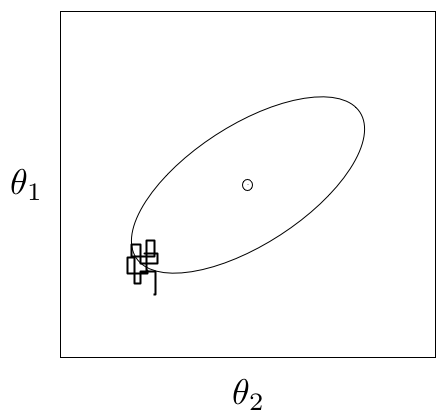
\includegraphics[height=3in]{poor_mixing.png}
\caption{An example of a poorly-mixing sample in two dimensions. Notice that the chain is trapped in a region of low probability relative to the mean (dot) and variance (oval) of the true posterior quantity.}
\label{fig:mix}
\end{center}
\end{figure}

\subsection*{Informal Methods}

The most straightforward approach for assessing convergence is based on
simply plotting and inspecting traces and histograms of the observed MCMC
sample. If the trace of values for each of the stochs exhibits asymptotic
behaviour\footnote{Asymptotic behaviour implies that the variance and the
mean value of the sample stays relatively constant over some arbitrary
period.} over the last $m$ iterations, this may be satisfactory evidence
for convergence. A similar approach involves plotting a histogram for every
set of $k$ iterations (perhaps 50-100) beyond some burn in threshold $n$;
if the histograms are not visibly different among the sample intervals,
this is reasonable evidence for convergence. Note that such diagnostics
should be carried out for each stoch estimated by the MCMC algorithm,
because convergent behaviour by one stoch does not imply evidence for
convergence for other stochs in the analysis. An extension of this approach
can be taken when multiple parallel chains are run, rather than just a
single, long chain. In this case, the final values of $c$ chains run for
$n$ iterations are plotted in a histogram; just as above, this is repeated
every $k$ iterations thereafter, and the histograms of the endpoints are
plotted again and compared to the previous histogram. This is repeated
until consecutive histograms are indistinguishable.

\begin{figure}[h]
\begin{center}
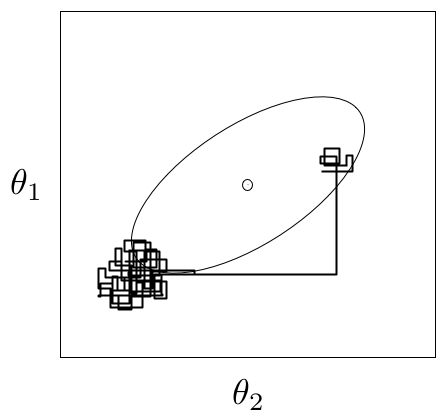
\includegraphics[height=3in]{metastable.png}
\caption{An example of metastability in a two-dimensional stoch space. The chain appears to be stable in one region of the stoch space for an extended period, then unpredictably jumps to another region of the space.}
\label{fig:metas}
\end{center}
\end{figure}

Another \emph{ad hoc} method for detecting convergence is to examine the traces of several MCMC chains initialized with different starting values. Overlaying these traces on the same set of axes should (if convergence has occurred) show each chain tending toward the same equilibrium value, with approximately the same variance. Recall that the tendency for some Markov chains to converge to the true (unknown) value from diverse initial values is called \emph{ergodicity}. This property is guaranteed by the reversible chains constructed using MCMC, and should be observable using this technique. Again, however, this approach is only a heuristic method, and cannot always detect lack of convergence, even though chains may appear ergodic.

A principal reason that evidence from informal techniques cannot guarantee convergence is a phenomenon called metastability. Chains may appear to have converged to the true equilibrium value, displaying excellent qualities by any of the methods described above. However, after some period of stability around this value, the chain may suddenly move to another region of the stoch space (Figure \ref{fig:metas}). This period of metastability can sometimes be very long, and therefore escape detection by these convergence diagnostics. Unfortunately, there is no statistical technique available for detecting metastability.

\subsection*{Formal Methods}

Along with the \emph{ad hoc} techniques described above, a number of more formal methods exist which are prevalent in the literature. These are considered more formal because they are based on existing statistical methods, such as time series analysis.

PyMC includes one formal convergence diagnostic method, first proposed by \citet{Geweke:1992gm}. This is a time-series approach, which compares the mean and variance of segments from the beginning and end of a single chain.
\begin{equation}
z = \frac{\bar{\theta}_a - \bar{\theta}_b}{\sqrt{Var(\theta_a) + Var(\theta_b)}}
\end{equation}
where $a$ is the early interval and $b$ the late interval. If the z-scores of these two segments are similar, it can provide evidence for convergence. PyMC plots the z-scores of the difference between various initial segments along the chain, and the last 50\% of the remaining chain. If the chain has converged, the majority of points should fall within 2 standard deviations of zero. Calling the convergence method results in a diagnostic plot for each model stoch.

\subsubsection{Method Usage}
\begin{verbatim}
sampler.convergence(first=0.1, last=0.5, intervals=20, burn=0, thin=1, chain=-1, plot=True)
\end{verbatim}
\begin{itemize}

\item \verb=first= (optional): First portion of chain to be used in Geweke diagnostic. Defaults to 0.1 (i.e. first 10% of chain).

\item \verb=last= (optional): Last portion of chain to be used in Geweke diagnostic. Defaults to 0.5 (i.e. last 50% of chain).

\item \verb=intervals= (optional): Number of sub-chains to analyze. Defaults to 20.

\item \verb=burn (optional)=: Number of burn-in iterations to exclude. Defaults to 0 (\emph{i.e.} no burn-in).

\item \verb=thin (optional)=: Thinning factor. Defaults to 1 (\emph{i.e.} no thinning).

\item \verb=chain= (optional): Chain to be analyzed. Defaults to -1 (\emph{i.e}. last chain).

\item \verb=plot= (optional): Plotting flag. Defaults to True.
\end{itemize}
Comprehensive convergence diagnostics are available in the \href{http://lib.stat.cmu.edu/R/CRAN/}{R statistical package}, via the \href{http://www-fis.iarc.fr/coda/}{CODA module}. The \verb=MetropolisHastings= class in PyMC includes a method for exporting model traces in a format that may be directly read by CODA.

\subsubsection{Method Usage}
\begin{verbatim}
sampler.coda_output(filename="coda", burn=0, thin=1)
\end{verbatim}
\begin{itemize}

\item \verb=filename= (optional): Filename of coda output files. Defaults to ``coda''.

\item \verb=burn (optional)=: Number of burn-in iterations to exclude. Defaults to 0 (\emph{i.e.} no burn-in).

\item \verb=thin (optional)=: Thinning factor. Defaults to 1 (\emph{i.e.} no thinning).

\end{itemize}
Calling \verb=coda_output= yields a \verb=.out= file containing raw trace values and a \verb=.ind= file containing indices.

% section convergence_diagnostics (end)

\section{Autocorrelation Plots} % (fold)
%\label{sec:autocorrelation_plots}

Samples from MCMC algorithms are ususally autocorrelated, due partly to the inherent Markovian dependence structure. The degree of autocorrelation can be quantified using the autocorrelation function:
\begin{eqnarray*}
    \rho_k &=& \frac{\mbox{Cov}(X_t, X_{t+k})}{\sqrt{\mbox{Var}(X_t)\mbox{Var}(X_{t+k})}} \\
            &=& \frac{E[(X_t - \theta)(X_{t+k} - \theta)]}{\sqrt{E[(X_t - \theta)^2] E[(X_{t+k} - \theta)^2]}}
\end{eqnarray*}
The \verb=MetropolisHastings= class includes a method for plotting the autocorrelation function for each stoch in the sampler (Figure \ref{fig:autocorr}). This allows users to examine the relationship among successive samples within sampled chains. Significant autocorrelation suggests that chains require thinning prior to use of the posterior statistics for inference.

\begin{figure}[h]
        \begin{center}
        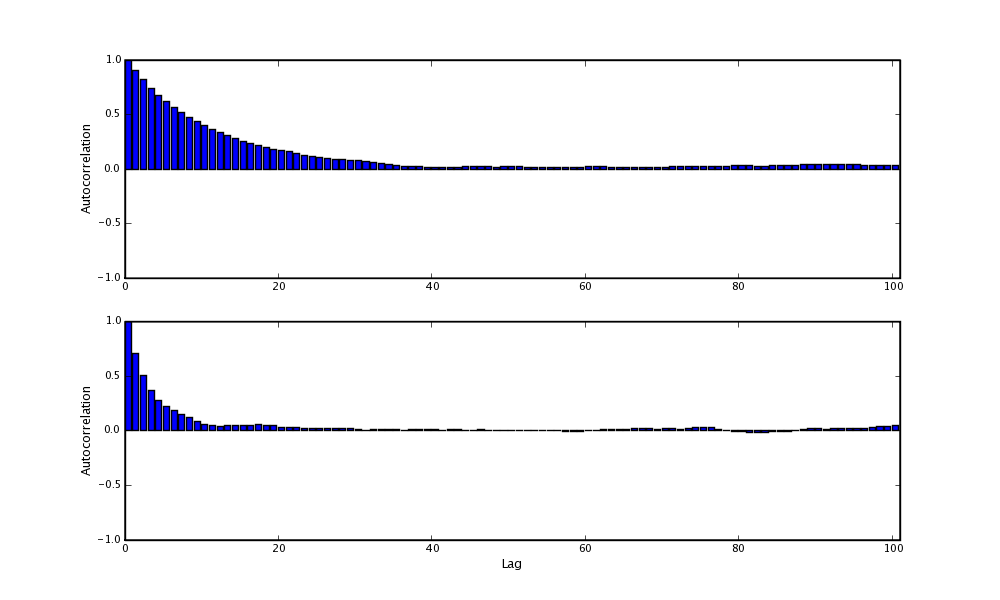
\includegraphics[scale=0.4]{autocorr.png}
    \end{center}
    \caption{Sample autocorrelation plots for two Poisson stochs from coal mining disasters example model.}
    \label{fig:autocorr}
\end{figure}

\begin{verbatim}
sampler.autocorrelation(max_lag=100, burn=0, thin=1, chain=-1)
\end{verbatim}

\begin{itemize}

\item \verb=max_lag (optional)=: Maximum time lag to calculate autocorrelation. Defaults to 100 iterations.

\item \verb=burn (optional)=: Number of burn-in iterations to exclude. Defaults to 0 (\emph{i.e.} no burn-in).

\item \verb=thin (optional)=: Thinning factor. Defaults to 1 (\emph{i.e.} no thinning).

\item \verb=chain (optional)=: Chain to be analyzed. Defaults to -1 (\emph{i.e}. last chain).
\end{itemize}

% section autocorrelation_plots (end)


\section{Goodness of Fit} % (fold)
%\label{sec:goodness_of_fit}


% section goodness_of_fit (end)